\documentclass[11pt, a4paper]{article}

\usepackage[left=2cm, top=3cm, text={17cm, 24cm}]{geometry}
\usepackage[T1]{fontenc}
\usepackage[czech]{babel}
\usepackage[utf8]{inputenc}
\usepackage{graphicx}
\usepackage[unicode, colorlinks, hypertexnames=false, citecolor=red]{hyperref}
\usepackage[htt]{hyphenat}
\usepackage{xcolor}
\usepackage{amsmath}
\usepackage{amsthm}
\usepackage{nameref}
\usepackage{parskip} % hezčí odsazení odstavců
\usepackage{float} % for using H for figures
\usepackage{subcaption} %subfigure
\setlength{\marginparwidth}{2cm}
\usepackage{todonotes}


\graphicspath{{img/}}

\theoremstyle{definition}
\newtheorem{definition}{Definice}[section]

\hypersetup{
    pdftitle={Umělá inteligence pro Válku kostek},
    pdfauthor={Josef Kolář; Dominik Harmim; Petr Kapoun; Jindřich Šesták}
}


\begin{document}


\begin{titlepage}
    \begin{center}
        \LARGE{\textsc{Vysoké učení technické v~Brně}} \\
        \smallskip
        \Large{\textsc{Fakulta informačních technologií}} \\

        \vspace{\stretch{.382}}

        \LARGE{SUI\,---\,Umělá inteligence a~strojové učení} \\
        \smallskip
        \Huge{Umělá inteligence pro Válku kostek} \\

        \vspace{\stretch{.618}}
    \end{center}

    \Large{%
        \begin{tabular}{l l r}
            \textbf{Josef Kolář} & \textbf{(\texttt{xkolar71})} & \\
            Dominik Harmim & (\texttt{xharmi00}) & \\
            Petr Kapoun & (\texttt{xkapou04}) & \\
            Jindřich Šesták & (\texttt{xsesta05}) & \hspace{9em} \today
        \end{tabular}
    }
\end{titlepage}


\pagenumbering{roman}
\setcounter{page}{1}
\tableofcontents
\clearpage


\pagenumbering{arabic}
\setcounter{page}{1}

\section{Úvod}

Cílem projektu bylo vytvořit \emph{umělou inteligenci (AI)} pro hru
\textbf{Válka kostek}. Umělá inteligence musí \emph{prohledávat stavový
prostor} hry a~musí využívat \emph{strojové učení}. Projekt je postaven
na bakalářské práci~\cite{turecekBP}\footnote{Projekt je konkrétně
založen na upravené verzi z~původní bakalářské
práce: \url{https://github.com/ibenes/dicewars}.}.

Dokumentace je dále strukturována následovně. Kapitola~\ref{sec:ai}
pojednává o~základní implementaci umělé inteligence založené na prohledávání
stavového prostoru hry. Kapitola~\ref{sec:aiMl} popisuje rozšíření
implementace o~prvky strojového učení. Vyhodnocení výsledné umělé
inteligence a~srovnání použitých přístupů je popsáno v~kapitole~\ref{sec:eval}.
Kapitola~\ref{sec:files} vysvětluje obsah odevzdávaného archivu. Konečně
kapitola~\ref{sec:con} shrnuje výsledky tohoto projektu.


\section{Implementace umělé inteligence prohledáváním stavového prostoru}
\label{sec:ai}

Po analýze prostředí a~implementace hry bylo zjištěno, že prostředí je
\emph{plně pozorovatelné} a~\emph{stochastické}. Na základě těchto
vlastností bylo nejdříve uvažováno o~implementaci umělé inteligence
jako \emph{agenta} (agent reprezentuje jednoho hráče), který bude
implementovat \emph{prohledávání stavového prostoru} algoritmem
$ ExpectiMiniMax $ popsaným v~původní bakalářské práci~\cite{turecekBP}.
Tento algoritmus vychází z~algoritmu $ MiniMax $. Je však rozšířen
o~\emph{nedeterministické} akce, proto je vhodný pro toto stochastické
prostředí.

Algoritmus $ MiniMax $ i~$ ExpectiMiniMax $ je však ve své standardní
variantě definován pouze pro hru dvou hráčů. V~tomto projektu je
nutné uvažovat hru čtyřech (a~obecně~$ n $) hráčů. Existuje zobecnění
těchto algoritmů pro hru~$ n $ hráčů. Jedná se o~tzv. $ Max^n $ algoritmus,
který lze opět rozšířit o~nedeterminismus. Dále bude hovořeno pouze
o~$ Max^n $ algoritmu, ale ve výsledné implementaci tohoto projektu byl
patřičně rozšířen i~o~nedeterministické akce. Algoritmus $ Max^n $ byl
poprvé představen v~článku \emph{An Algorithmic Solution of N-Person
Games}~\cite{nPersonGames}, kde je podrobně popsán spolu s~problematikou her
pro více hráčů. Článek \emph{Comparison of Algorithms for Multi-player
Games}~\cite{compMultiPlGames} pak srovnává algoritmus $ Max^n $
s~alternativními algoritmy pro hry více hráčů.

\subsection{\texorpdfstring{Algoritmus $ Max^n $}{Algoritmus MaxN}}
\label{subsec:algoritmus-max-n}

Algoritmus $ Max^n $ je přesně definován ve výše uvedených
článcích~\cite{nPersonGames, compMultiPlGames}, proto bude v~této kapitole už
jen neformálně popsán a~znázorněn.

V~klasickém algoritmu $ MiniMax $ se střídají tahy dvou hráčů. Hráč na
tahu\,---\,$ MAX $\,---\,se snaží vybírat tahy vedoucí do stavů s~maximálním
ohodnocením, tj. snaží se maximalizovat svoji \emph{objektivní funkci}.
Protihráč\,---\,$ MIN $\,---\,se naopak snaží minimalizovat objektivní funkci
hráče $ MAX $. Tyto dvě hodnoty lze reprezentovat jednou hodnotu
vytvořením jejich sumy. Je také možné dívat se na tento problém tak, že
každý z~hráčů se snažím maximalizovat svoji vlastní objektivní
funkci. Potom by se dalo při prohledávání stavového prostoru tohle
reprezentovat jako dvojice maximálních hodnot objektivní funkce pro
každého z~hráčů.

Algoritmus $ Max^n $ potom funguje stejně jako $ MiniMax $, kde se ale
při prohledávání uvažuje $ n $-tice, kde~$ n $ je počet hráčů. Každý prvek
této $ n $-tice reprezentuje maximalizovanou hodnotu objektivní funkce
daného hráče a~každý z~hráčů se snaží svoji objektivní funkci při svém
tahu maximalizovat. Algoritmus je ilustrován na obrázku~\ref{fig:maxn}.
Uvažuje se hra pro~3 hráče\,---\,A, B, C. Tito hráči se v~uvedeném pořadí
střídají při hraní svých tahů. Každý z~hráčů může provést dva možné tahy.
Po třech tazích hra skončí (obecně by po tahu hráče~C hrál opět hráč~A,
ale zde jsou tahy hráče~C uvažovány jako koncové, po nichž hra končí).
Stav hry je tady popsán trojicí\,---\,$ (obj(\text{A}), obj(\text{B}),
obj(\text{C})) $\,---\,kde $ obj(\text{X}) $ je hodnota objektivní funkce
hráče~X. Na obrázku je vidět expandovaný graf hry pro dané hráče. Listové
uzly jsou ohodnoceny objektivní funkcí a~nelistové uzly jsou ohodnoceny
podle maximalizace objektivní funkce aktuálního hráče na tahu. Je zřejmé,
že hráč~A učiní tah \uv{vpravo}, protože stav, do kterého tento tah vede,
je ohodnocen pro něho nejlepší objektivní funkcí\,---\,$ (1, 1, 1) $.
Cesta do koncového stavu s~tímto ohodnocením je vyznačena červenými hranami.

\begin{figure}[H]
    \centering
    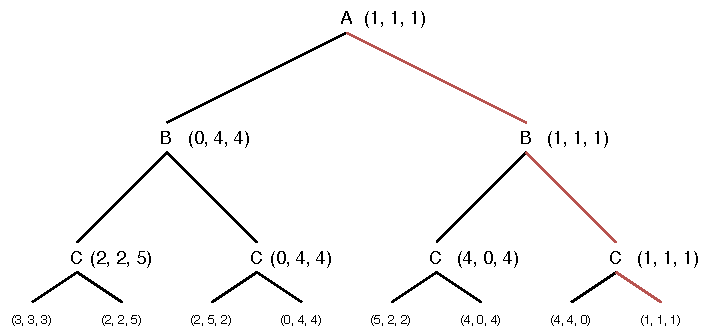
\includegraphics[width=.8 \linewidth]{maxn.pdf}
    \caption{%
        Příklad \emph{prohledávání stavového prostoru} hry pro~3 hráče
        algoritmem $ Max^n $%
    }
    \label{fig:maxn}
\end{figure}

\subsection{\texorpdfstring{%
    Konkrétní implementace a~použití algoritmu $ Max^n $%
}{Konkrétní implementace a~použití algoritmu MaxN}}
\label{subsec:implementce-a-pouziti-algoritmu}

Tato kapitola popisuje výslednou implementaci umělé inteligence
prohledáváním stavového prostoru algoritmem $ Max^n $ pro tento projekt.
Dále popisuje rozšíření tohoto algoritmu o~nedeterministické akce
a~konkrétní použití v~projektu.

Implementace prohledávání stavového prostoru se nachází ve třídě
\texttt{dicewars.ai.xkolar71.AI} (kromě implementace heuristické funkce
pro ohodnocování stavů hry, která je implementována ve třídě
\texttt{dicewars.ai.xkolar72\_orig.AI}, vzhledem k~tomu, že heuristická funkce
byla nakonec nahrazena strojově učeným modelem, viz kapitola~\ref{sec:aiMl}).

\medskip

\begin{definition}[$ maxN $]
Byla definována \emph{rekursívní} funkce $ maxN $, která implementuje
algoritmus $ Max^n $ pro účely tohoto projektu. Funkce v~každém tahu daného
hráče zkoumá následující tahy všech ostatních hráčů v~patřičném pořadí
a~vrací nejlepší spočítaný tah. Funkce konkrétně uvažuje~$ n $ iterací
prohledávání tahů všech následujících hráčů. Parametr~$ n $ byl
experimentálně zvolen na hodnotu~$ 1 $, tj. uvažuje se nanejvýše jedenkrát
sekvence tahů každého z~následujících hráčů. Při vyšších hodnotách tohoto
parametru už byly naměřeny horší výsledky, což je způsobené tím, že prostředí
hry je \emph{silně nedeterministické} a~jen obtížně lze přesněji predikovat
výsledky akcí dále do budoucnosti. Při zkoumání tahů hráče následujícího
v~pořadí se generuje~$ m $ útoků. Následně z~každého útoku se generuje
$ m - 1 $ útoků, z~každého z~nich $ m - 2 $ útoků atd. až do hloubky~$ l $.
Parametry~$ m $ a~$ l $ byly experimentálně nastaveny na hodnotu~5, opět
s~ohledem na stochastické prostředí. Útoky, které se generují v~daném
tahu, jsou vybrány jako ty možné útoky s~\emph{největší pravděpodobností} na
výhru funkcí $ possibleTurns $, viz definice~\ref{def:possTurns}. Tímto
byl algoritmus $ Max^n $ rozšířen o~nedeterminismus. Uvažované útoky jsou
vždy simulovány na kopii aktuální konfigurace hry. Funkce $ maxN $ potom
v~listových uzel (definovaných parametry~$ n $ a~$ l $) ohodnotí daný stav
\emph{heuristickou funkcí}~$ h $, viz definice~\ref{def:h}. Konečně $ maxN $
maximalizuje hodnotu funkce~$ h $ pro každého z~hráčů a~vrací tah do uzlu
s~nejlepším ohodnocením.
\end{definition}

\medskip

\begin{definition}[$ possibleTurns $]
\label{def:possTurns}
Tato funkce vrací všechny tahy, které je možné provést seřazené podle
\emph{pravděpodobnosti}~$ p $. Tahy, které je možné provést, jsou
všechny možné útoky (tj. útoky z~území, na nichž jsou alespoň 2~kostky
a~sousedí s~územím protihráče), jejichž pravděpodobnost~$ p $
je větší než 0,4 (bylo zvoleno experimentálně) a~nebo je počet kostek
na útočícím území roven 8 (největší možný počet kostek na území).
Pravděpodobnost~$ p $ je spočtena následovně $ p = P_{A \rightarrow D}
\cdot P_D \cdot P_L $, kde $ P_{A \rightarrow D} $ je pravděpodobnost
úspěšného útoku z~území~$ A $ na území~$ D $, $ P_D $ je pravděpodobnost
udržení území~$ D $ po úspěšném útoku při tazích následujících hráčů
a~$ P_L $ je~2 (zvoleno experimentálně) v~případě, že území~$ A $ leží
v~největším regionu daného hráče, tj. je proveden útok z~největšího území
hráče, v~opačném případě je $ P_L = 1 $. Výpočty těchto pravděpodobností
jsou blíže diskutovány v~původní bakalářské práci~\cite{turecekBP}.
\end{definition}

\medskip

\begin{definition}[$ h $]
\label{def:h}
Hodnota této \emph{heuristické funkce} udává ohodnocení stavu hry pro
každého hráče ve smyslu maximalizace jeho \emph{objektivní funkce}.
Hodnota~$ h $ pro hráče~$ i $ je spočtena následovně $ h(i) = D(i) +
\sum_r^{R(i)} 5 r + 50 \max (R(i)) $, kde~$ D(i) $ je počet kostek
hráče~$ i $, $ R(i) $ jsou velikosti regionů hráče~$ i $ a~číselné konstanty
byly zvoleny experimentálně.
\end{definition}

Na nejvyšší úrovni je tah hráče určen tak, že pokud je zbývající časové
omezení tahu větší než~$ x $ sekund a~zároveň je počet tahů v~aktuální sérii
tahů daného hráče menší než~$ y $, tak se nalezne nejlepší tah funkcí
$ maxN $. V~opačném případě se vybere nejlepší možný útok s~ohledem na
pravděpodobnost výhry funkcí $ possibleTurns $. Pokud žádný takový útok
není možný, tah se ukončí. Parametry~$ x $ a~$ y $ byly experimentálně
nastaveny na hodnoty~1,0 a~5.


\section{Strojově učený model pro heuristickou funkci}
\label{sec:aiMl}

Model substituuje \emph{heuristickou funkci} a~pro každého hráče vyhodnocuje v~rámci aktuální konfigurace hry jeho šanci na výhru.
Vstupem je tedy serializace aktuální konfigurace hry (stavu desky a~stavu hráčů) do XX celých čísel a~výstupem je vektor~4 hodnot v~intervalu $<0;1>$, který udává odhad modelu na výhru jednotlivých hráčů; $0$ značí, že model si je jistý s~nevýhrou hráče s~konkrétním indexem (resp. jménem).

\subsection{Serializace hry}
\label{sec:serialiseGame}

Pro trénování modelu jsme navrhli serializaci hry do vektoru XX celých čísel, který odpovídá konkrétnímu stavu hry, tedy desky a~hráčů na ní hrajících. Výsledný vektor má následující strukturu:

\begin{itemize}
    \item matice sousednosti $M_s$ definovaná jako
    \begin{align*}
        M_s =
        \begin{bmatrix}
            s(1, 1) & s(1, 2) & s(1, 3) & \ldots & s(1, 29) \\
            \cdot   & s(2, 2) & s(2, 3) & \ldots & s(2, 29) \\
            \cdot   & \cdot   & s(3, 3) & \ldots & s(3, 29) \\
            \cdot   & \cdot   & \cdot   & \ldots & s(4, 29) \\
            \cdot   & \cdot   & \cdot   & \cdot  & \ldots   \\
            \cdot   & \cdot   & \cdot   & \cdot  & s(29, 29)\\
        \end{bmatrix}
    \end{align*}
    kdy funkce $s(x, y)$ je definovaná následovně
    \begin{equation*}
        s(x, y) =
        \begin{cases}
            1 & \text{jestliže území}\ x\ \text{sousedí s územím}\ y\\
            0 & \text{jinak}\\
        \end{cases}
    \end{equation*}
    a výsledný vektor sousednosti je poté získán jako konkatenace řádků $M_s$ z trojúhelníku nad diagonálou. Jeho celková délka je $\frac{30 * (30 - 1)}{2} = 435$ prvků.
    \item vlastníci polí\,---\,tedy vektor o délce $30$ s hodnotami, resp. názvy, jednotlivých vlastníků polí, opět $30$ prvků
    \item počtů kostek\,---\,vektor udávající množství kostek pro každé pole na desce
    \item velikosti největších regionů\,---\,vektor o délce $4$ s $max(R(i))$ pro každého hráče $i$
\end{itemize}

Serializovaná hra je tedy vektor celočíselných nezáporných čísel složený ze čtyř sektorů s celkovou délkou $435 + 30 + 30 + 4 = 499$ prvků.

Po každém ukončeném tahu hráče je uschována serializace hry.
Po konci hry je ke všem serializacím přiložen index vítěze konkrétní posloupnosti tahů a~tento datový balíček
je binárně uložen na disk. Pro tento účel byla upravena metoda \texttt{run} třídy \texttt{Game}, která se nachází v~modulu
\texttt{dicewars.server.game}. Pro tuto serializaci se dále používají funkce z~vytvořeného modulu
\texttt{dicewars.ml}.

\subsection{Trénování modelu neuronové sítě}
\label{sec:trainModel}

\textit{Všechny skripty zmíněné v~této sekci se nachází v~adresáři \texttt{ml-scripts}}.

Čtyřikrát původní AI s~$ Max^n $ algoritmem, souborový systém se soubory s~jednotlivými konfiguracemi. Pro finální natrénování modelu bylo použito 201\,291 různých konfigurací her s~odpovídajícími indexy vítězů. Pro generování konfigurací byla hra spuštěna vytvořeným skriptem \texttt{dump-data-to-learn.py}.

Pomocí skriptu \texttt{transform-to-numpy.py} je tato datová sada ze souborů transformována na pole typu \texttt{numpy} o~dimenzích $(N, 1 + 499)$\,---\,$N$ značí celkový počet konfigurací a~$1 + 499$ je index vítěze a~kompletní serializace hry. Takto zkonstruované pole je uloženo jako jeden samostatný soubor pro další zpracování.

Implementace dalšího zpracování datové sady je pak v~souboru \texttt{shuffle-datasets.py}, který ji načte, náhodně zamíchá podle první dimenze (tedy pořadí různých konfigurací) a~následně rozdělí na \emph{trénovací}, \emph{validační} a~\emph{testovací} data. To dělá v~poměru 70\,\%, 20\,\% a~zbylých 10\,\% pro testovací data. Takto rozdělená sada je následně uložena do třech samostatných souborů.

Trénovací a~validační část datové sady je následně použita pro natrénování modelu (skript \texttt{train-model.py})\,---\,tím je v~tomto případě \emph{lineární neuronová síť}. Její architektura byla zvolena experimentálně a celkově se skládá z pěti vrstev,
z čehož první vrstva je čistě vstupní se vstupním vektorem o délce 499 (délka vychází ze způsobu serializace). Následuje plně propojená vrstva s 64 parametry a ReLU aktivací, jako třetí figuruje v síti \texttt{Dropout} vrstva pro prevenci přeučení s pravděpodobností vynulování vstupů $p=0.25$ a model je zakončen dvěma plně propojenými vrstvami s 32, resp. 4 parametry. Čtvrtá vrstva používá opět aktivaci ReLU, výstupní poté \texttt{softmax}. Níže je přiložen programový výstup z \texttt{keras} popisu modelu. 

\begin{verbatim}
__________________________________________________
Layer (type)          Output Shape        Param #
==================================================
input_1 (InputLayer)  [(None, 499)]       0
__________________________________________________
dense (Dense)         (None, 64)          32000
__________________________________________________
dropout (Dropout)     (None, 64)          0
__________________________________________________
dense_1 (Dense)       (None, 32)          2080
__________________________________________________
dense_2 (Dense)       (None, 4)           132
==================================================
Total params: 34,212
Trainable params: 34,212
Non-trainable params: 0
__________________________________________________
\end{verbatim}

Nutno zmínit, že v~případě předpokládaných výsledků pro každou konfiguraci dochází ke \emph{kategorizaci}\,---\,transformaci celočíselného indexu vítěze na vektor o~počtu hráčů s~hodnotou $1$ na místě indexu vítěze a~hodnotami $0$ na ostatních pozicích\,---\,tedy platí, že pro vítěze s indexem $i$ je modelu předložen předpokládaný vektor $\begin{bmatrix}
  x_1 & x_2 & x_3 & x_4 \\ 
\end{bmatrix}$ u kterého platí, že $x_i = 1$, a $0$ jinak.

Pro samotné natrénování je použit algoritmus \texttt{Adam} pro optimalizátor s~\emph{learning rate} na hodnotě $0,01$. Jako \emph{loss} pak trénování používá instanci \texttt{CategoricalCrossentropy} dodanou přímo knihovnou \texttt{keras}.
Jako velikost trénovací i~validační dávky jsme experimentálně stanovili hodnotu $32$ a~počet epoch jsme opět experimentálně nastavili na $15$.

Pro ověření správnosti modelu jsme připravili skript \texttt{check-test-accuracy.py}, který určí přesnost odhadů nad částí datové sady určenou pro testování (tedy 10\,\% z~původní sady). Natrénovaný model z~testovací datové sady o~velikosti
20\,130 správně určil celkem 19\,804 vzorků, což značí úspěšnost cca $98.3\,\%$.

Pro ověření rychlosti vyhodnocení modelu pro vstupní data jsme připravili skript \texttt{profile-predict.py}, s pomocí kterého jsme za asistence \texttt{CProfile} profileru měřili rychlost vyhodnocení. Pro výše definovanou síť a testovací část datové sady bylo experimentálně změřeno první vyhodnocení cca 1,5 násobně delší, než ty následující (tedy 550\,ms oproti 350\,ms)\,---\,což je známý a popsaný problém modelů založených na Tensorflow\footnote{\url{https://github.com/tensorflow/tensorflow/issues/39458}}.

\subsection{Integrace modelu}
\label{subsec:model-integration}
Pro použití natrénovaného modelu v~AI je upravena heuristická funkce, která nyní na základě předané konfigurace hry vyhodnocuje jednotlivé hráče, resp. jejich šanci na vítězství. Konkrétně se jedná o funkci \texttt{\_heuristic(players: List[int], board: Board)}, která na základě předaného seznamu aktivních hráčů a instance desky provede nejprve serializaci (dle postupu popsaného výše), následně vyhodnotí konfiguraci v natrénovaném modelu a nazpět vrátí ohodnocení stavu hry pro jednotlivé hráče\,---\,konkrétní hodnota pro hráče odpovídá maximalizaci jeho \emph{objektivní funkce}.

\section{Vyhodnocení implementace umělé inteligence}
\label{sec:eval}

Po prvotní implementaci algoritmu $ Max^n $ pro účely umělé inteligence pro tuto hru jsme začali experimentovat s hraním soutěžních turnajů, kterých se účastnila i tato inteligence. Do turnajů jsme zapojovali umělé inteligence dle zadání výsledného soutěžního turnaje, tedy \texttt{dt.ste},  \texttt{dt.wpm\_c}, \texttt{dt.sdc}, \texttt{xlogin00} a nakonec i \texttt{xkolar71}. Po prvotním odladění parametrů (popsaných v kapitole \ref{subsec:implementce-a-pouziti-algoritmu}) na základě experimentů
se turnajová úspěšnost pohybovala mezi 35\,\% a 60\,\%\,---\,viz výsledky turnajů zobrazených v \ref{fig:vysledky-turnaje-bez-modelu}.

S prvními výsledky po implementaci algoritmu $ Max^n $ jsme vygenerovali serializace konfigurací her určené pro natrénování modelu, jak je popsáno v \ref{sec:trainModel}, a natrénovaný model následně integrovali do umělé inteligence, konkrétně do její heuristické funkce (jak popisuje \ref{subsec:model-integration}). Nad takto upravenou umělou inteligencí jsme spustili další turnaje, z nichž naše umělá inteligence vycházela s úspěšností na úrovni umělé inteligence bez integrace modelu\,---\,na základě tohoto pozorování jsme iterativně vylepšovali trénování modelu (experimentální změny architektury sítě, konkrétní struktury serializovaných her či velikostí datových sad). 

Tyto iterace změn vedly ve výsledku k úspěšnosti umělé inteligence s integrovaným modelem na úrovni stabilních 39\,\% až 43\,\% na turnajích s násobně vyššími počty her (nad 1000). Výsledky z některých turnajů jsou zobrazeny v \ref{fig:vysledky-turnaje-s-modelem} a nutné je poznamenat, že AI \texttt{xkolar71} s integrovaným modelem vycházela z těchto turnajů úspěšněji než verze AI \texttt{xkolar71\_orig}, která je původní implementací bez integrovaného modelu.

\begin{figure}[H]
    \centering
    \begin{subfigure}{\textwidth}
        \centering
        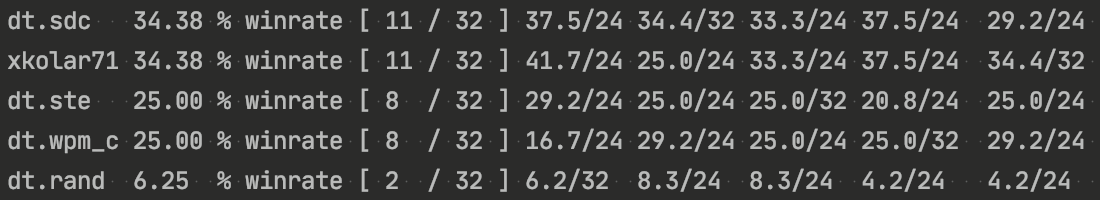
\includegraphics[width=\linewidth]{tournament-1.png}
        \vspace{0mm}
    \end{subfigure}
    \begin{subfigure}{\textwidth}
        \centering        
        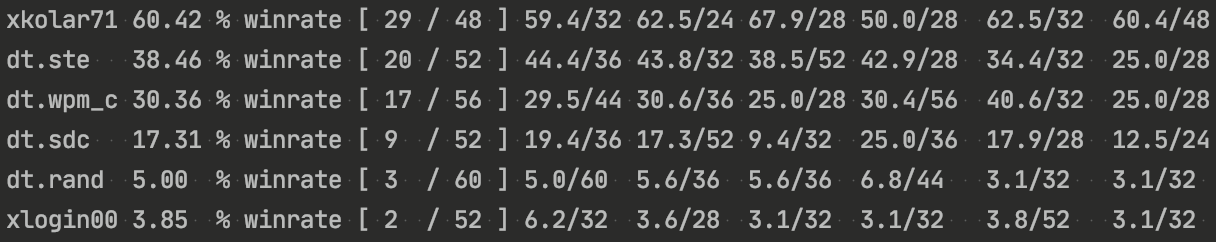
\includegraphics[width=\linewidth]{tournament-3.png}
        \vspace{0mm}
    \end{subfigure}
    \begin{subfigure}{\textwidth}
        \centering
        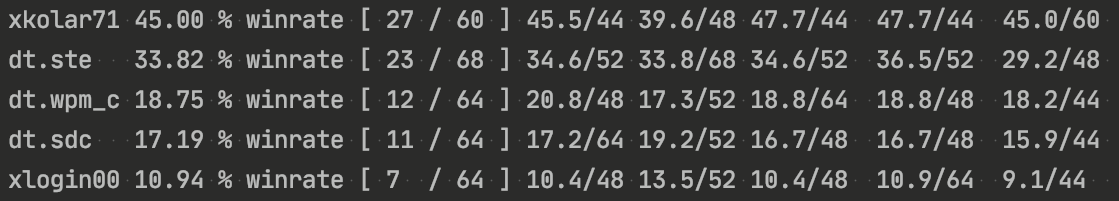
\includegraphics[width=\linewidth]{tournament-2.png}
    \end{subfigure}
    \caption{Výsledky soutěžních turnajů po prvotní implementaci umělé inteligence\,---\,tedy bez strojového učení.}
    \label{fig:vysledky-turnaje-bez-modelu}
\end{figure}


\begin{figure}[H]
    \centering
    \begin{subfigure}{\textwidth}
        \centering
        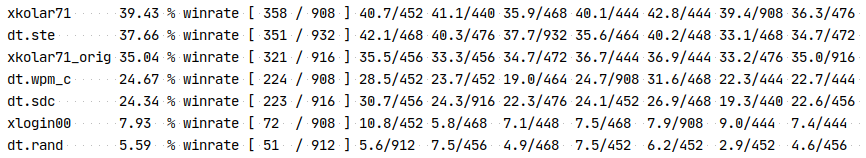
\includegraphics[width=\linewidth]{tournament-nn-1.png}
        \vspace{0mm}
    \end{subfigure}
    \begin{subfigure}{\textwidth}
        \centering        
        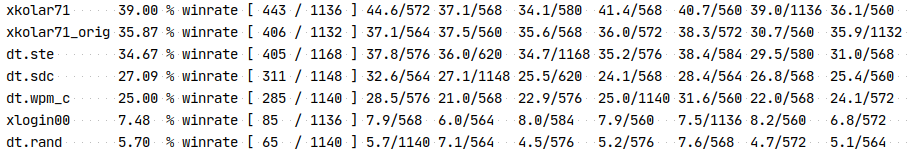
\includegraphics[width=\linewidth]{tournament-nn-2.png}
        \vspace{0mm}
    \end{subfigure}
    \begin{subfigure}{\textwidth}
        \centering
        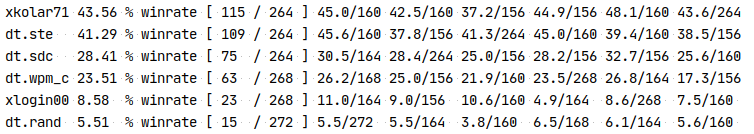
\includegraphics[width=\linewidth]{tournament-nn-3.png}
    \end{subfigure}
    \caption{Výsledky soutěžních turnajů po integraci naučeného modelu\,---\,tedy se strojovým učením.
    AI \texttt{xkolar71\_orig} značí umělou inteligenci bez integrovaného modelu.}
    \label{fig:vysledky-turnaje-s-modelem}
\end{figure}

\section{Obsah odevzdaného archivu}
\label{sec:files}

Odevzdaný archiv \texttt{xkolar71.zip} obsahuje následující soubory:
\begin{itemize}
    \item
        \texttt{xkolar71/\_\_init\_\_.py}
        a~\textcolor{blue}{\texttt{xkolar71/ai.py}}: Balíček,
        který obsahuje implementaci umělé inteligence, která \emph{používá
        strojové učení}. Viz kapitola~\ref{sec:aiMl}.

    \item
        \texttt{xkolar71/model.h5}: Natrénovaný model založený
        na \emph{neuronové síti}, který se používá pro modelování
        \emph{heuristické funkce} pro ohodnocování stavů hry.
    
    
    \item
        \texttt{xkolar71/game.py}: Modul s implementací serializační
        funkce popsané v kapitole \ref{sec:serialiseGame}.

    \item
        \texttt{supplementary/dicewars/ai/xkolar71\_orig.py}: Původní implementace umělé
        inteligence \emph{bez strojového učení} popsaná
        v~kapitole~\ref{sec:ai}.

    \item
        \texttt{supplementary/dicewars/ai/xkolar71\_2.py},
        \texttt{supplementary/dicewars/ai/xkolar71\_3.py},
        \texttt{supplementary/dicewars/ai/xkolar71\_4.py}: \\
        Další instance původní implementace umělé inteligence
        \texttt{supplementary/xkolar71\_orig} vytvořené pro účely trénování modelu.

    \item
        \texttt{supplementary/dicewars/server/game.py}: Modifikovaný soubor s~třídou, která
        řídí hru. Byla provedena úprava pro generování konfigurací hry za
        účelem trénování modelu. Viz kapitola~\ref{sec:serialiseGame}.

    \item
        \texttt{supplementary/dicewars/ml/\_\_init\_\_.py} a~\texttt{supplementary/dicewars/ml/game.py}:
        Balíček obsahující funkce sloužící k~serializaci konfigurací hry.
        Viz kapitola~\ref{sec:serialiseGame}.

    \item
        \texttt{supplementary/ml-scripts/dump-data-to-learn.py}: Skript pro generování
        konfigurací hry. Viz kapitola~\ref{sec:trainModel}.

    \item
        \texttt{supplementary/ml-scripts/transform-to-numpy.py}: Skript pro převod
        vygenerovaných konfigurací hry na pole typu \texttt{numpy}. Viz
        kapitola~\ref{sec:trainModel}.

    \item
        \texttt{supplementary/ml-scripts/shuffle-datasets.py}: Skript pro zamíchání
        konfigurací hry a~jejich následné rozdělení na \emph{trénovací},
        \emph{validační} a~\emph{testovací} datové sady. Viz
        kapitola~\ref{sec:trainModel}.

    \item
        \texttt{supplementary/ml-scripts/train-model.py}: Skript pro vytvoření a~trénování
        modelu založeném na neuronové síti. Viz kapitola~\ref{sec:trainModel}.

    \item
        \texttt{supplementary/ml-scripts/check-test-accuracy.py}: Skript pro ověření
        správnosti modelu na testovacích datech. Viz
        kapitola~\ref{sec:trainModel}.
        
    \item
        \texttt{supplementary/ml-scripts/profile-predict.py}: Skript pro ověření
        rychlosti predikce na testovacích datech. Viz
        kapitola~\ref{sec:trainModel}.


    \item
        \texttt{requirements.txt}: Aktualizovaný seznam knihoven, na
        kterých je projekt závislý.

    \item
        \texttt{xkolar71.pdf}: Tato dokumentace k~projektu.
\end{itemize}


\section{Závěr}
\label{sec:con}

V rámci řešení tohoto projektu jsme po úvodním rozdělení práce nastudovali funkci algoritmu $ Max^N $, abychom jej mohli následně implementovat a experimentálně nastavit jednotlivé parametry pro jeho běh -- samotná funkce algoritmu je stručně popsána v kapitole \ref{sec:ai} a to včetně popisu konkrétní implementace a jednotlivých parametrů. Po prvotní implementaci dosahovala umělá inteligence míry výher pohybujících nad úrovní 30\,\%, ve většině případů na prvním místě spouštěných turnajů.

Takto chovající se umělá inteligence byla následně použita (resp. čtyři identické její instance) pro vygenerování trénovací a validační datové sady, podle kterých byl poté natrénován model ze třívrstvé neuronové sítě -- tento proces včetně architektury sítě a trénovacího \emph{workflow} je popsán v kapitole \ref{sec:aiMl}. Po integraci do původního algoritmu pomocí substituce heuristické funkce se míra výher nové umělé inteligence pohybovala nad 35\,\% a i nadále na prvních pozicích desítek soutěžních turnajů.

Závěrem této dokumentace je výčet souborů v odevzdaném archivu včetně popisu funkce jednotlivých skriptů pro možnou replikovatelnost.

% \section{Inspirace}

% \subsection{Kombinace algoritmu a~NN}
% \url{https://www.semanticscholar.org/paper/A-hybrid-neural-network-and-Minimax-algorithm-for-Plessis/2eadbea2748bfb8097e06f5d2dd64dde3be840dd}\\
% \url{https://www.sciencedirect.com/science/article/pii/S0004370201000935}\\
% \url{https://www.semanticscholar.org/paper/Improving-heuristic-mini-max-search-by-supervised-Buro/8ac607a3147ad384c66f2f138d44b42ae951a0be}\\
% \url{http://citeseerx.ist.psu.edu/viewdoc/download?doi=10.1.1.97.7820&rep=rep1&type=pdf}\\
% \url{https://www.sciencedirect.com/science/article/abs/pii/S0031320304002365}\\
% \url{https://ai.stackexchange.com/questions/12020/minimax-combined-with-machine-learning-to-determine-if-a-path-should-be-explored}\\
% \url{https://stackoverflow.com/questions/753954/how-to-program-a-neural-network-for-chess}\\
% \url{https://courses.engr.illinois.edu/cs440/sp2019/slides/hockenmaier12.pdf}\\
% \url{https://lib.dr.iastate.edu/cgi/viewcontent.cgi?article=1491&context=creativecomponents}\\
% \url{://github.com/lukemun/ShallowBlue}\\
% \url{https://digitalcommons.lsu.edu/cgi/viewcontent.cgi?article=1766&context=gradschool_theses}\\
% \url{https://scialert.net/fulltext/?doi=itj.2012.1655.1659}\\
% \url{https://books.google.cz/books/about/AI_2008_Advances_in_Artificial_Intellige.html?id=fSA1HKsw9tsC&redir_esc=y} strana 73 a~dale \\
% \url{https://ieeexplore.ieee.org/document/1347290}\\
% \url{http://nn.cs.utexas.edu/downloads/papers/moriarty.focus.pdf}\\

% \subsection{AlphaZero}
% \url{https://deepmind.com/research/open-source/alphazero-resources}\\
% \url{https://science.sciencemag.org/content/362/6419/1140}\\
% \url{https://arxiv.org/abs/1910.13012}\\
% \url{https://arxiv.org/abs/2009.04374}\\
% \url{https://arxiv.org/abs/1712.01815}\\
% \url{https://www.chess.com/news/view/new-alphazero-paper-explores-chess-variants}\\


% \newpage
\bibliographystyle{czplain}
\bibliography{xkolar71}


\end{document}
